\documentclass[12pt, a4paper]{article}

\usepackage[utf8]{inputenc}
\usepackage[italian]{babel}
\usepackage[T1]{fontenc}
\usepackage{parskip}
\usepackage{helvet} 
\usepackage{xcolor}
\pagecolor[rgb]{0.1, 0.1, 0.1} 
\color[rgb]{0.9, 0.9, 0.9}
\usepackage{amsmath, amssymb, amsthm}
\usepackage{mathtools}
\usepackage{graphicx} 
\usepackage{forest}
\usetikzlibrary{mindmap, trees, arrows.meta, positioning, shapes}
\usepackage{listings}

\lstset{
    frame=none,     
    basicstyle=\ttfamily\small\color[rgb]{0.9, 0.9, 0.9},
    keywordstyle=\color[rgb]{0.4, 0.7, 1.0},
    commentstyle=\color[rgb]{0.4, 0.6, 0.4},
    stringstyle=\color[rgb]{1.0, 0.6, 0.4},
    breaklines=true,
    escapeinside={[$$]}{[$$]}, 
    escapebegin={$},           
    escapeend={$}
}

\forestset{
  default preamble={
    for tree={
      draw=gray,
      fill=rgb:red,0.2;green,0.2;blue,0.2,
      rounded corners,
      node options={align=center},
      font=\sffamily\small,
      edge={color=gray, line width=1pt}
    }
  }
}
\usepackage{tikz}
\usetikzlibrary{arrows.meta, automata, positioning, shapes}
\usepackage[left=2cm, right=2cm, top=2cm, bottom=2cm]{geometry}

\begin{document}

\title{Intelligenza artificiale}
\author{Giorgio Poluzzi}
\maketitle

\section{AI-problem-solving}

\subsection{Agents and environments}

Gli agenti sono entità che percepiscono l'ambiente. La funzione degli agenti è mappare le percezioni in azioni.
$$
f:P^*\to A
$$
Il programma dell'agente viene elaborato su una struttura fisica producendo $f$.

Se un agente possiede $\left|P\right|$ percezioni, allora il numero di entrate possibili sarà
$$
\sum_{t=1}^T \left|P\right|^t
$$
Lo scopo dell'AI è quello di progettare piccoli programmi che rappresentino funzioni complesse.

\subsubsection*{Esempio}
% breadboard: bb1
\begin{lstlisting}
function Reflex-Vacuum-Agent([locatiom.status]) returns an action
         if status = Dirty then return Suck
         else if location = A then return Right
         else if location = B then return Left
\end{lstlisting}
% end breadboard

\subsection{Rationality}
Un agente razionale sceglie quale azione massimizza il valore atteso della misura della performance, data la sequenza di percezioni passate.

Le percezioni non devono essere provviste di tutte le informazioni rilevanti.

I risultati delle azioni potrebbero non essere sempre prevedibili.

La razionalizzazione dei risultati delle azioni dipende dall'esplorazione, dall'autonomia e da ciò che l'agente ha appreso.

\subsubsection*{Esercizio}
\begin{itemize}
  \item L'ambiente è composto da tre stanze (A, B, C) e due robot (r1, r2).
  
  \item Il robot r1 può pattugliare le stanze A e B, mentre r2 può pattugliare le stanze B e C.
  
  \item Alla partenza, r1 si trova nella stanza A e r2 si trova nella stanza C.
  
  \item Il tempo di viaggio necessario per spostarsi tra le stanze è pari a zero.
  
  \item La misura di prestazione da ottimizzare è la minimizzazione della somma dell'ozio medio (average idleness) di tutte le stanze.
  
  \item L'ozio medio è definito come la somma degli intervalli di tempo in cui una stanza non è visitata da alcun robot, divisa per il tempo totale.
\end{itemize}  

L'esercizio chiede di identificare quale sarebbe un comportamento razionale per questo specifico ambiente.

Dal momento che un robot può pattugliare contemporaneamente solo una stanza, ci sarà sempre una stanza vuota.

Bisogna minimizzare l'ozio totale, minimizzando il numero di stanze vuote nel tempo.

Se i robot pattugliano una stanza ciascuno, la stanza B sarà vuota, ma se entrambi pattugliano B, allora ci saranno due stanze vuote.

Un comportamento razionale sarebbe quello di far pattugliare A ad r1 e C a r2.

\subsection{Peas}

Per progettare un agente razionale, bisogna specificare la missione dell'ambiente.

Il tipo di ambiente determina in gran parte l'architettura dell'agente.

\subsection{Problem types}

I tipi di problema possibili sono:
\begin{itemize}
  \item Deterministico, totalmente osservabile $\to$ single-state problem
  \item Non osservabile $\to$ conformant problem
  \item Non deterministico, parzialmente osservabile $\to$ contingency problem
  \item Stato dello spazio non conosciuto $\to$ exploration problem
\end{itemize}

\subsection{Problem-solving agents}

I goal-based agents sono agenti che scelgono le azioni da compiere in base allo stato dell'ambiente, cercano una soluzione e eseguono la soluzione ignorando le percezioni (approccio offline).

% breadboard: bb2
\begin{lstlisting}
function Simple-Problem-Solving-Agent(percept) returns an action
static: seq, an action sequence, initially empty
        state, some description of the current world state
        goal, a goal, initially null
        problem, a problema formulation
state <- Update-State(state, percept)
if seq is empty then
   goal <- Formulate-Goal(state)
   problem <- Formulate-Problem(state,goal)
   seq<-Search(problem)
action <- First(seq)
seq <- Rest(seq)
return action
\end{lstlisting}
% end breadboard

\subsubsection*{Esempio}

Holiday in Romania:

Formulare un goal:
\begin{itemize}
  \item andare a Bucharest
\end{itemize}
Formulare un problema: 
\begin{itemize}
  \item states: various cities
  \item actions: drive between cities
\end{itemize}
Trovare una soluzione:
\begin{itemize}
  \item trovare un percorso che metta le città in sequenza
\end{itemize}

\begin{figure}[h]
  \centering
  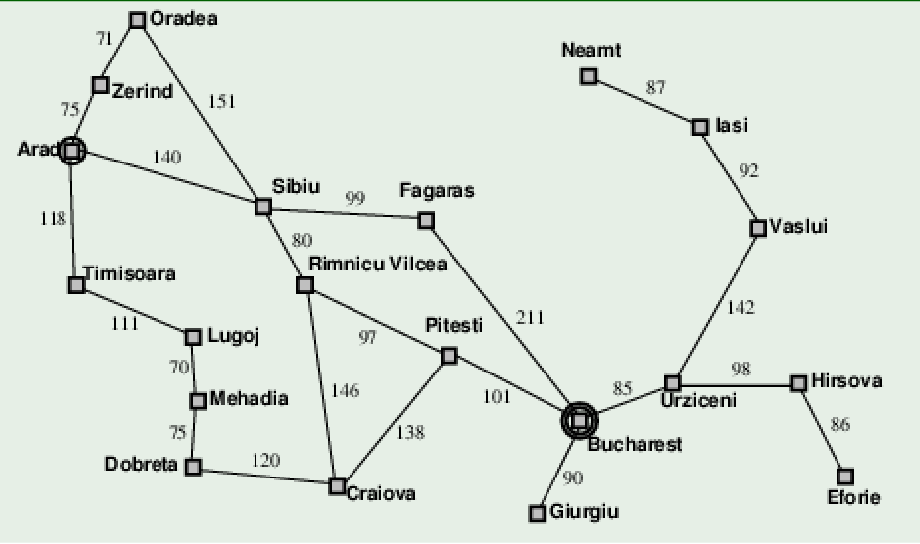
\includegraphics[width=0.8\textwidth]{img/2026-10-09_10-08-26.png}
  \caption{}
  \label{fig:2026-10-09_10-08-26}
\end{figure}

% breadboard: bb3
\begin{lstlisting}
initial state = Arad
successor function S(x) = set of action-state pairs
                          {<Arad->Zerind,Zerind>,...}
goalt test
      explicit x=Bucharest
      implicit NoDirt(x)
path cost(additive)
     sum of distances, number of actions excecuted
     c(x,a,y) is the step cost (>=0)
solution
     sequence of actions leading from initial state to goal
\end{lstlisting}
% end breadboard

\subsection{Tree search algorithm}

% breadboard: bb4
\begin{lstlisting}
function Tree-Search(problem,strategy) return solution or failure
initialize the search tree using the initiale state of problem
loop do
     if no candidates for expansion then return failure
choose a leaf node for expansion according to strategy
if node contains a goal state then return a solution
add successor nodes to the search tree (expansion)
end
\end{lstlisting}
% end breadboard

\subsection{State vs Nodes}
Uno stato è una rappresentazione di una configurazione fisica dell'ambiente

Un nodo è un dato strutturale che costituisce una parte dell'alber di ricerca, e include parent, action, children, depth, path cost... .

Gli stati invece non contengono nodi figli, parenti ecc...

\begin{figure}[h]
  \centering
  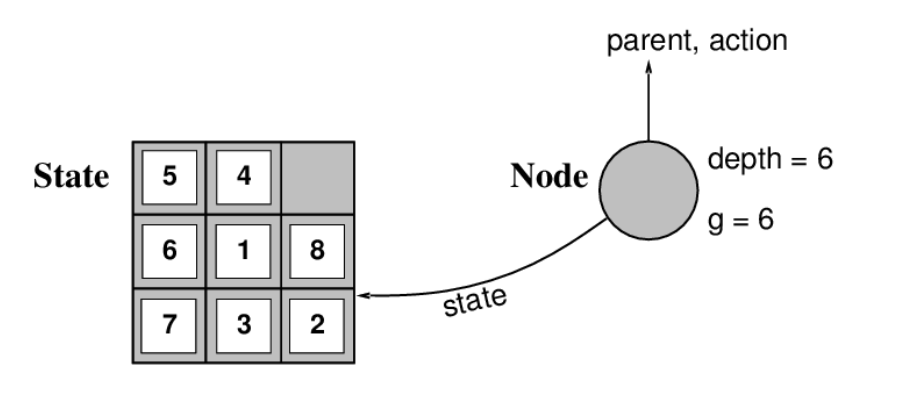
\includegraphics[width=0.8\textwidth]{img/2026-10-09_10-18-04.png}
  \caption{}
  \label{fig:2026-10-09_10-18-04}
\end{figure}

\subsection{General Tree Search}

% breadboard: bb5
\begin{lstlisting}
function Tree-Search(problem,frontier) returns a solution or failure
frontier <- Inser(Make-Node(problem.Initial-State))
while not isEmpty(frontier) do
      node <- Pop(frontier)
      if problem.Goal-Test(node.State) then return node
      frontier <- InsertAll(Expand(node,problem))
end loop
return failure
\end{lstlisting}
% end breadboard

\subsection{Implementation: Expand Nodes}
% breadboard: bb6
\begin{lstlisting}
function Expand(node,problem) return a set of nodes
successors <- the empty set
for each action, result in Successor-Fn(problem,node.State) do
    s <- a new Node
    s.Parent.Node <- node;
    s.Action <- action
    s.State <- result
    s.Path-Cost <- node.Path-Cost + Ste-Cost(node.State,action,result)
    s.Depth <- node.Depth+1
    add s to successors
return successors
\end{lstlisting}
% end breadboard

Ovviamente per la ricerca si applicano delle strategie in base a completezza di tempo, di problema, di spazio, di ottimalità.

La complessità di tempo e spazio è misurata da:
\begin{itemize}
  \item b: maximum branching factor of the search tree
  \item d: depth of the least-cost solution
  \item m: maximum depth of the state space (may be $\infty$)
\end{itemize}

\subsection{Graph Search}
% breadboard: bb7
\begin{lstlisting}
function Grapth-Search(problema,frontier) return a solution, or failure
explore <- an empty set
frontier <- Insert(Make-Node(problem.Initial-State))
while not IsEmpty(frontier) do
      node <- Pop(frontier)
      if problem.Goal-Test(node.State) the return node
      if node.State is not in explored then
        add node.State to explored
        frontier <- InsertAll(Expand(node,problem)
      end if
end loop
return failure
\end{lstlisting}
% end breadboard


\section{Local Search}
\subsection{Iterative improvement algorithms}
Nella maggior parte dei problemi di ottimizzazione, il percorso è irrilevante, ciò che conta è raggiungere l'obiettivo.

Lo state space è un set completo di configurazioni.

\subsection{Hill-Climbing}
% breadboard: bb8
\begin{lstlisting}
function Hill-Climbing(problem) returns a state that is a local maximum
         inputs: problem, a problem
         local variables: current, a node
                          neighbor, a node

         current <- Make-Node(problem.Initial-State)
         loop do
              neighbor <- a highest-valued successor of current
              if neighbour.Value <= current.Value then return
                 current.State
              end if
              current <- neighbor
         end
\end{lstlisting}
% end breadboard

% breadboard: bb9
\begin{lstlisting}
function Simulated-Annealing(problem,schedule) returns a solution state
         inputs: problem, a problem
                 schedula, a mapping fromm time to "temperature"
         local variables: current, a node
                          next, a node
                          T, a "temperature" controlling prob. of downward steps

         current <- Make-Node(problem.Initial-State)
         for t <- 1 to infty do
             T <- schedule(t)
             if T = 0 then return current
             next <- a random selected successor of current
             \Delta E <- next.Value - current.Value
             if \Delta E > 0 then current <- next
             else current <- next only with probability $e^{\frac{\Delta E}{T}}$
\end{lstlisting}
% end breadboard

\section{Local Search in continuous spaces}

\subsection*{Example}

\subsubsection*{Placing airports in Romania}

Si vogliono posizionare tre aeroporti per minimizzare la somma del quadrato delle distanze tra ogni città e l'aeroporto più vicino.

\begin{itemize}
  \item Airport location: $(x_1, y_1), (x_2, y_2), (x_3, y_3)$
  \item City location: $(x_c, y_c)$
  \item $C_a$ cities closest to airport $a$ $a = \{1,2,3\}$
\end{itemize}

Minimizzazione oggettiva:
$$
\sum_a{\sum_{c\in C_a}(x_a-x_c)^2+(y_a-y_c)^2}
$$

\subsection{Discretizzazione}

È un metodo che trasforma uno spazio continuo in uno spazio discreto, così da poter applicare gli algoritmi di ricerca locale.

\begin{itemize}
  \item fix $\delta$
  \item si considera una variazione di $\pm\delta$ in ogni cordinata
  \item si utilizza un qualsiasi algoritmo di ricerca locale discreto
\end{itemize}

La prima scelta ricade sull'algoritmo di Hill-Climbing fino a quando una variazione casuale non migliora lo stato corrente.

Si utilizza il simulated annealing per evitare di rimanere bloccati in un massimo locale.

Si calcola infine il gradiente di $f(X)$ analiticamente ($X=\{x_1,\dots,x_n\}$)

\subsection{Calcolo del gradiente}

$
\nabla f(X) = 
\left(
  \frac{\partial f}{\partial x_1},
  \frac{\partial f}{\partial x_2},
  \dots,
  \frac{\partial f}{\partial x_n}
\right)
$

Sull'esempio dell'aeroporto, si calcola come segue:
$
f(X) = \sum_a{\sum_{c\in C_a}(x_a-x_c)^2+(y_a-y_c)^2}
$

e $X = \{x_1,y_1,x_2,y_2,x_3,y_3\}, n=6$

\begin{itemize}
  \item $\frac{\partial f}{\partial x_1}=\sum_{c\in C_1}2(x_1-x_c)$
  \item per trovare l'estremo si risolve per $\nabla f(X) = 0$
  \item risolvere in locale
\end{itemize}

\subsection{Local gradient}

Spesso non è possibile risolvere $\nabla f(X) = 0$ in maniera analitica globalmente, ma si può risolvere localmente.

\begin{itemize}
  \item Si prova a proseguire il calcolo per ogni coordinata in direzione positiva salendo lungo il gradiente.
  \item Più è alta la pendenza (quindi più la derivata è grande), più è probabile che la direzione sia quella giusta.
\end{itemize}

Si consideri una funzione generica a due variabili $g(x_1,x_2)$, la si aggiorni per il metodo del gradiente.

$
x_1\leftarrow x_1 + \alpha \times \frac{\partial g(x_1,x_2)}{\partial x_1}, x_2\leftarrow x_2 + \alpha \times \frac{\partial g(x_1,x_2)}{\partial x_2}
$

Si proceda con la notazione vettoriale

\begin{align*}
  X & = [x_1, x_2]^T, \nabla g(X) =[\frac{\partial g}{\partial x1}, \frac{\partial g}{\partial x2}]^T \\
  X &\leftarrow X + \alpha \times \nabla g(X)
\end{align*}

$\alpha$ è la grandezza del passo, una costante positiva di basso valore, è fondamentale trovare un valore ottimale per $\alpha$.

Se $\alpha$ è troppo grande, si rischia di saltare alcune soluzioni ottimali, se è troppo piccolo, si rischia di effettuare troppi passi e impiegare troppo tempo per raggiungere la soluzione.

\subsection{Newton Raphson}

Il metodo di Newton-Raphson è un metodo iterativo per trovare le radici di diversi problemi di local search in uno spazio continuo.

La tecnica generica consiste nel trovare le radici di una funzione $f(x)$, quindi si risolve $f(x) = 0$.

Scegliere un valore iniziale di $\overline{x}_0$

Aggiornare progressivamente la stima di $\overline{x}_{n+1}=\overline{x}_n-\frac{g(\overline{x_n})}{g'(\overline{x_n})}$

dove $g'(x)=\frac{\partial g(x)}{dx}$ è la derivata della funzione $g(x)$.

\subsection*{Aplpicazione del metodo di Newton-Raphson}

Si consideri la funzione $g(x)=x^2-a$

Si dimostri che il metodo di Newton porta alla soluzione ricorsiva cos' definita:
$$
  x_{n+1}=\frac{1}{2}
  \left ( 
    x_n + \frac{a}{x_n}  
  \right )
$$
  
Si imposti $a=4, x_0=1$ e si calcoli $x_i$ con $i\in\{1,2,3\}$

$\square$

\subsection{Interpretazione geometrica del metodo di Newton}

Si assuma $y=f(x)$ con radice $x=r$ che sia tangente al punto $(a,f(a))$ con funzione $y=f(a)+(x-a)f'(a)$

Sia $b$ la intercetta per la retta tangente, $0=f(a)+(x-a)f'(a)$ si ricava: $b=a-\frac{f(a)}{f'(a)}$

b è la nuova stima della radice per il metodo di Newton-Raphson partendo da $a$.

Per trovare un estremo per f(X) bisogna trovare $\overline(X)$ tale che $\nabla f(\overline{X})=0$

È possibile utilizzare il metodo di Newton-Raphson dove $g(X)$ è la derivata di $f(X)$, quindi $\nabla f(X)$

In forma di matrice vettoriale, l'aggiornamento di Newton-Raphson diventa:

\begin{align*}
  x & \leftarrow x - H_f^{-1}(x)\nabla f(x) \\
  H_{ij} &= \frac{\partial^2 f}{\partial x_i \partial x_j}
\end{align*}

Per problemi di grandi dimensioni, calcolare $n^2$ valori della matrice Hessiana e invertire la matrice $N\times N$ potrebbe essere computazionalmente costoso. Si utilizzano quindi approsimazioni della matrice Hessiana.

A volte non si ha a disposizione la funzione $f(X)$. In quel caso si stima la pendenza sperimentalmente, calcolando le coordinate su valori diversi di $\pm\delta$ studiando come varia la funzione (in pratica un hill-climbing).

\section{CSP, Contrait Satisfaction Problem}

Assunzioni: singolo agente, azioni deterministiche, stato monitorabile, spazio discreto.

\subsubsection*{Planning}

\begin{itemize}
  \item Si vuole conoscere il percorso per raggiungere l'obiettivo,
  \item i percorsi hanno un costo associato,
  \item le euristiche specificano una guida alla risoluzione del probkema.
\end{itemize}

\subsubsection*{Identification}

\begin{itemize}
  \item L'unico elemento di interesse è la soluzione finale,
  \item la local search potrebbe tornare parecchio utile (ma la sua efficacia non è garantita), e può essere utilizzata anche in spazi continui.
  \item la CSP è una classe specializzata nell'identificazione dei problemi.
\end{itemize}

Un problema di ricerca standard può essere descritto in tal maniera:

\begin{itemize}
  \item Lo stato iniziale è definito da un qualsiasi insieme di variabili e valori (scatola nera),
  \item Il goal test può essere una qualsiasi funzione tra gli stati,
  \item La funzione di transizione (che mappa la funzione successiva) può essere una qualsiasi funzione che mappa lo stato corrente in un set di stati successivi.
\end{itemize}

\begin{itemize}
  \item Uno stato è definito da un set di variabili $X=X_i$ che possono assumere valori da un dominio $D=D_i$
  \item Il goal test è un set di vincoli che specificano le combinazioni di valori ammissibili per un sottoinsieme di variabili,
  \item Si possono utilizzare strategie di risoluzione generiche che sfruttano queste caratteristiche che risultano più efficienti ed efficaci delle strategie tradizionali.
\end{itemize}

\subsection*{Example}

Si piazzino $N$ regine su una scacchiera con $N\times N$ caselle in maniera che nessuna regina possa attaccare un'altra regina.

\begin{itemize}
  \item $X:\{x_{i,j}\},i\in\{1,\dots,N\},j\in\{1,\dots,N\}$: si ottiene così una sola variabile per ogni cella della scacchiera
  \item $D:\{D_{i,j}\},D_i\in0,1$: dominio di valori ammissibili booleano (0=false, 1=true)
  \item $\forall{i,j,k}(X_{i,j},X_{i,k})\in\{(0,0),(0,1),(1,0)\}$ soltanto una regina per ogni riga.
  \item $\forall{i,j,k}(X_{i,j},X_{k,j})\in\{(0,0),(0,1),(1,0)\}$ soltanto una regina per ogni colonna.
  \item $\forall{i,j,k}(X_{i,j},X_{i+k,j+k})\in\{(0,0),(0,1),(1,0)\}$ soltanto una regina su ogni diagonale (a dx)
  \item $\forall{i,j,k}(X_{i,j},X_{i+k,j-k})\in\{(0,0),(0,1),(1,0)\}$ soltanto una regina su ogni diagonale (a sx)
  \item $\sum_{i,j}X_{i,j} = N$
\end{itemize}

Si consideri solo una regina per ogni colonna

\begin{itemize}
  \item X: $\{x_i\},i\in\{1,\dots,N\}$: si ottiene così una sola variabile per ogni colonna della scacchiera
  \item D: $\{D_i\},D_i\in\{1,\dots,N\}$: riga per la regina nella colonna $i$
  \item $C:\{C_1,\dots,C_k\},k\in\{1,\dots,Nx(N-1)/2\}$ un vincolo per ogni coppia di variabili, che specifica le posizioni ammissibili delle due regine.
\end{itemize}

\subsection*{Per esempio}
\begin{figure}[h]
  \centering
  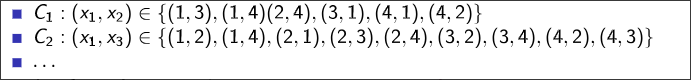
\includegraphics[width=0.8\textwidth]{img/2026-10-14_17-35-33.png}
  \caption{}
  \label{fig:2026-10-14_17-35-33}
\end{figure}

Questa formulazione rende alcuni vincoli impliciti, non è ad esempio possibile assegnare due regine alla stessa colonna, non bisogna eseguire un controllo.

\subsection*{Problemi di combinatoria}

Dato un set di possibili soluzioni, si cerca di trovare la migliore possibile. Le soluzioni sono tante, ma discrete e finite, una ricerca completa non è possibile.z



\section{Logical Agents}

\textbf{Knowledge base} = è un insieme di frasi scritte in linguaggio formale


\end{document}